%%%%%%%%%%%%%%%%%%%%%%%%%%%%%%%%%%%%%%%%%
% FRI Data Science_report LaTeX Template
% Version 1.0 (28/1/2020)
% 
% Jure Demšar (jure.demsar@fri.uni-lj.si)
%
% Based on MicromouseSymp article template by:
% Mathias Legrand (legrand.mathias@gmail.com) 
% With extensive modifications by:
% Antonio Valente (antonio.luis.valente@gmail.com)
%
% License:
% CC BY-NC-SA 3.0 (http://creativecommons.org/licenses/by-nc-sa/3.0/)
%
%%%%%%%%%%%%%%%%%%%%%%%%%%%%%%%%%%%%%%%%%


%----------------------------------------------------------------------------------------
%	PACKAGES AND OTHER DOCUMENT CONFIGURATIONS
%----------------------------------------------------------------------------------------
\documentclass[fleqn,moreauthors,10pt]{ds_report}
\usepackage[english]{babel}

\graphicspath{{fig/}}




%----------------------------------------------------------------------------------------
%	ARTICLE INFORMATION
%----------------------------------------------------------------------------------------

% Header
\JournalInfo{FRI Natural language processing course 2024}

% Interim or final report
\Archive{Project report} 
%\Archive{Final report} 

% Article title
\PaperTitle{LLM Prompt Strategies for Commonsense-Reasoning Tasks} 

% Authors (student competitors) and their info
\Authors{Žan Počkar, Amer Mujagić, and Ivan Nikolov}

% Advisors
\affiliation{\textit{Advisors: Aleš Žagar}}

% Keywords
\Keywords{Prompt Strategies, Prompt Evaluation}
\newcommand{\keywordname}{Keywords}


%----------------------------------------------------------------------------------------
%	ABSTRACT
%----------------------------------------------------------------------------------------

\Abstract{
In order to systematically evaluate and compare the efficiency of different prompt strategies, we developed a flexible testing framework capable of accommodating multiple prompting techniques and LLMs. We utilized the DSPy framework to reshape prompts from a selected dataset to align with the Chain-of-Thought strategy. We used Llama3 to generate predictions based on Chain-of-Thought prompts and zero-shot prompts on 100 examples from the Physical IQa dataset.
}

%----------------------------------------------------------------------------------------

\begin{document}

% Makes all text pages the same height
\flushbottom 

% Print the title and abstract box
\maketitle 

% Removes page numbering from the first page
\thispagestyle{empty} 

%----------------------------------------------------------------------------------------
%	ARTICLE CONTENTS
%----------------------------------------------------------------------------------------

\section*{Introduction}
Large Language Models (LLMs) have shown remarkable progress in various tasks when supplied with extensive training material. However, improving their commonsense reasoning capabilities remains a considerable challenge. Commonsense reasoning, which involves making judgments based on everyday knowledge and experiences, is a vital aspect of human intelligence. Incorporating this ability into LLMs is a complex task.

In this paper, we compare two prompting strategies Chain of Thought and Zero-Shot. Our evaluation framework, designed to accommodate multiple models and strategies in the future, uses a subset of the Physical IQa benchmark for testing. The primary objective of this paper is to serve as a proof of concept for our evaluation framework and to provide a blueprint for comparing the effectiveness of different prompt strategies on various LLMs.

%------------------------------------------------
\section*{Problem}

Commonsense reasoning in Large Language Models (LLMs) is a complex problem due to the implicit and context-dependent nature of commonsense knowledge. For instance, consider the sentence “The ice cream was too hot to eat.” Humans intuitively understand this sentence is likely incorrect because ice cream is typically cold. However, an LLM might not flag this as an anomaly unless it has been explicitly trained on similar examples or has learned to associate certain objects with their typical properties.

Another challenge is the representation and utilization of commonsense knowledge in LLMs. LLMs learn from the patterns in the data they are trained on, so the size and quality of the training dataset significantly influence their performance. However, encoding commonsense knowledge into a machine-readable format that an LLM can learn from is not straightforward. For example, understanding that “people usually sleep at night” requires the model to learn not just the concepts of “people,” “sleep,” and “night,” but also the typical association between these concepts.

Lastly, the evaluation of commonsense reasoning in LLMs is a significant challenge. Traditional evaluation metrics may not adequately capture the nuances of commonsense reasoning. For instance, if an LLM generates the sentence “The man opened his umbrella because it was raining,” it demonstrates an understanding of the causal relationship between rain and using an umbrella. However, quantifying this understanding and comparing it across different models or tasks is not trivial, necessitating the development of more sophisticated evaluation metrics and benchmarks.

Our approach to this implementation starts with taking the prompts from a given dataset and using an LLM to reshape them into a given strategy. Unfortunately not many datasets are available that compare different strategies and most are used to compare different LLMs. After reshaping the prompts we run them through the model and compare the results we get to the correct results from the dataset.

\section*{Prompting Techniques}

Prompts techniques are the proposed input structures that guide LLMs to produce outputs with the desired form and content quality. That is, to simplify, we can say that we use different prompting techniques to "program" LLM inputs by following specific patterns in order to obtain an output. \cite{prompttechniques}

\subsection*{Zero shot prompting}
Zero-shot prompting \cite{Few-shot} is a prompting technique in which the prompt is made up only of natural language instruction describing the task. Meaning that no additional demonstrations are allowed. An example of zero-shot, one-shot and few-shot learning, with each "shot" being an additional demonstration, can be seen in Figure \ref{fig:few-shot} 

\begin{figure}[!h]\centering
	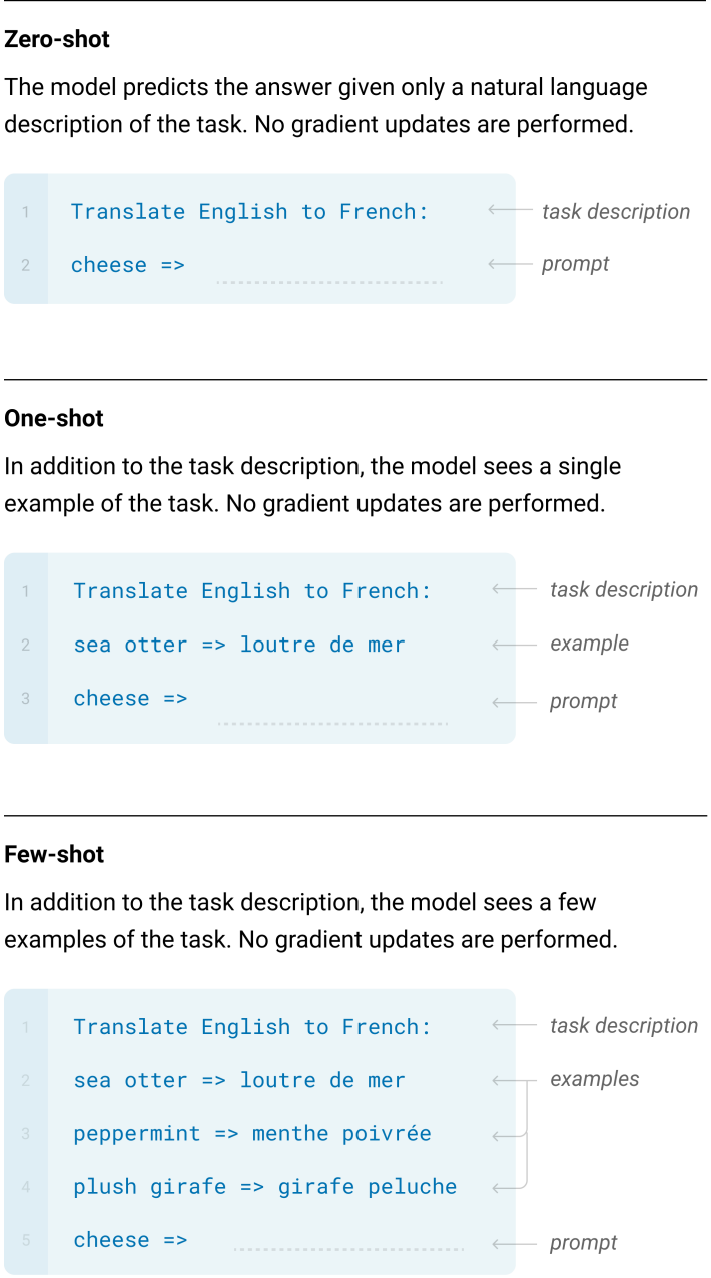
\includegraphics[width=\linewidth]{fig/few-shot-new.png}
	\caption{Examples of zero-shot, one-shot and few-shot prompts}
	\label{fig:few-shot}
\end{figure}

\subsection*{Chain of thought}
Chain of Thought (CoT) \cite{CoT} prompting involves adding a series of intermediate reasoning steps to the intended task. It has been shown to improve performance in more complex prompts.
These intermediate reasoning steps can be thought of as giving an answer to a similar problem but with detailed steps on how to get to that answer as shown in Figure 1. This is similar to few-shot prompting, which also provides examples of answers to similar questions, however few-shot prompts include less detail that is they usually provide only questions and answers, no intermediate reasoning steps in between. \cite{CoT}
An example of Chain of Thought prompting can be seen in Figure \ref{fig:cot}
\begin{figure}[!h]\centering
	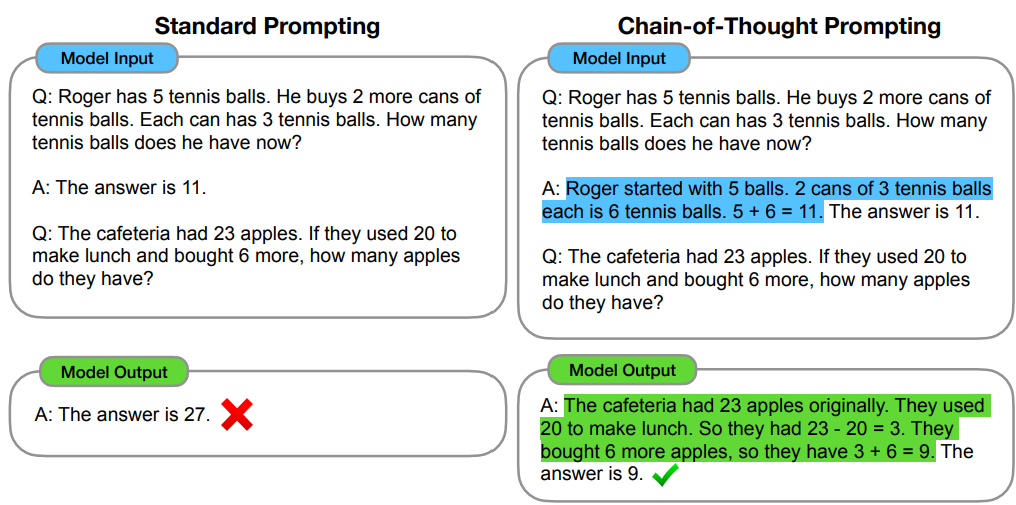
\includegraphics[width=\linewidth]{Example_CoT.png}
	\caption{Example of a Chain of Thought prompt versus a regular prompt}
	\label{fig:cot}
\end{figure}





\section*{Datasets}
Because commonsense reasoning is a complex topic and encompasses a wide collection of different tasks, it is difficult to generate a dataset that will evaluate the model's generalization abilities.

The Winograd schema challenge \cite{levesque2012winograd} was the standard for testing the commonsense reasoning, however from 2019 it is considered defeated since numerous transformer-based models achieved over 90\% accuracy. \cite{beaten_winograd}
For that reason, we will use more recent and challenging datasets.

On the one side, we have different SOTA methods \cite{CoT} evaluated on task specific datasets like GSM8K \cite{GSMK8}. This dataset focuses on linguistically diverse grade school math problems created by human problem writers.

On the other side, there are benchmarks that combine multiple commonsense datasets. For this project we will use Rainbow which is a suite of commonsense benchmarks that contain multiple choice question-answering datasets.
Rainbow contains the following datasets

\begin{itemize}
    \item $\alpha$NLI \cite{alphaNLI} - tests abductive reasoning in narratives. Models need to find the best explanation among the presented options connecting a beginning and ending;
    \item  CosmosQA \cite{Tian2020} — asks commonsense reading comprehensions about narratives in everyday situations
    \item HellaSWAG \cite{Zellers2020} — models need to find the most plausable ending to a short content.
    \item PIQA \cite{Bisk2020} — question answering benchmark for commonsense reasoning.
    \item SocialIQa \cite{socialIQA} — commonsense reasoning about social situations and interactions
    \item WinoGrande \cite{WinoGRANDE} — large-scale collection of Winograd schema-inspired problems that test reasoning about social and physical interactions.
\end{itemize}

Other possibilities for testing commonsense reasoning are the GLUE \cite{GLUE} and SuperGLUE \cite{supeglue} datasets, which are benchmarks for general language understanding systems.

\section{Results}

\subsection{Setup}
Our plan was to test our implementation on two promoting strategies. We used the DSPy framework \cite{dspy} to reshape prompts into CoT prompts,  and used the zero-shot prompts as a baseline. We generated predictions on a subset of 100 examples from the Physical IQa dataset using the Llama3-8B-instruct model.

\subsection{First results}
Initial results for the chain-of-thought prompting technique are promising. In a benchmark test where we provided the model with just the question, the model achieved approximately 55\% accuracy, which is only marginally better than guessing in datasets where the model is given a question and two possible answers. However, upon implementing the chain-of-thought technique, we observed a significant increase in accuracy, reaching over 70\%. This 15\% improvement is a notable achievement for our first and rudimentary implementation of the COT technique.


\section*{Evaluation}
We are currently performing evaluation of the models answers with two different methods. In the first method where the model has to select between two choices and then give his answer we use a simple comparison algorithm. If the model gives multiple answers, we count up the choices and use his most often given answer as the answer we use for comparison. The comparison algorithm is then a simple checker which has the list of correct answers. The checker compares the question id and content from the correct list with those give by the model. And then prints the results.

The other comparison method is a much more involved process for when the model gives a descriptive answer. In this method, we are using an uncased BERT model to generate the embedding and calculate the cosine similarity between the correct answer and the given one. As an additional layer of grading we are comparing cosine similarity with Word2Vec model to better determine the meaning of the sentence these two scores are then combine and if the answer pass the threshold of correctness we are considering the answer as correct. This model also supports comparison of different techniques, and not just direct comparison between the result and the technique. This way we can determine which technique is closer to the right answer even if this particular answer is incorrect.

\section{Discussion}
In spite of the promising results, we encountered a challenge related to increased run times when employing the chain-of-thought technique, even on an HPC cluster. We attribute this issue mainly to the current implementation's inefficiency. Addressing this inefficiency will be a key focus in refining the chain-of-thought approach for real-world applications.
As our main goal is to compare multiple prompt strategies, our next steps will be implementing additional strategies and additional models and creating a detailed analysis of the final results.

 
%----------------------------------------------------------------------------------------
%	REFERENCE LIST
%----------------------------------------------------------------------------------------
\bibliographystyle{unsrt}
\bibliography{report}


\end{document}